\documentclass[twocolumn]{report}
\usepackage{graphicx}
\newcommand{\ident}{\indent}
\newcommand{\acos}{\cos^{-1}}
\newcommand{\asin}{\sin^{-1}}
\newcommand{\atan}{\tan^{-1}}
\newcommand{\acosh}{\cosh^{-1}}
\newcommand{\asinh}{\sinh^{-1}}
\newcommand{\ve}[1]{\overrightarrow{\mathbf{#1}}}

\newenvironment{changemargin}[2]{%
\begin{list}{}{%
\onecolumn%
\setlength{\leftmargin}{#1}%
\setlength{\rightmargin}{#2}%
}%
\item[]}{\end{list}}

\newenvironment{twocol}[0]{%
\begin{list}{}{%
\onecolumn
\setlength{\leftmargin}{0cm}%
\setlength{\rightmargin}{0cm}%
}%
\item[]}{\end{list}}


\begin{document}
\title{
\begin{center}
\textbf{Reflections implementation}\end{center}
\begin{center}
\textbf{For}\end{center}
\begin{center}
\textbf{D3D9Client}\end{center}
\vspace{-2cm}
}
\maketitle
\begin{twocol}

\section*{Fresnel reflection}

Fresnel reflection will occur when a ray of light will hit into an "optical" material that has a refractive index $n$. Good examples of such materials are glass, water and most plastics. Fresnel reflection is highly depended from a viewing angle. In the D3D9Client we use so called Schlick's approximation of fresnel reflection. 

\begin{equation}
 R = R_0 + (1-R_0)(1-\cos\theta)^p
\end{equation}

Where the "Offset" $R_0$ is given by
\begin{equation}
R_0 = \left[\frac{1-n}{1+n}\right]^2
\end{equation}

To gain some additional properties for our function we have replaced the term $(1-R_0)$ with a multiplier $m$ resulting an equation

\begin{equation}
 R = R_0 + m(1-\cos\theta)^p
\end{equation}

Here are two plots of the equation using different values of $p$. Red curve is using value 2.0 and blue 4.0. The parameter $p$ will only effect in the view angle dependency of the fresnel reflection. The multiplier $m$ is most often set to a value $1-R_0$ and in that case the maximum reflection intensity is 1.0.

\begin{figure}[h]
	\centering
	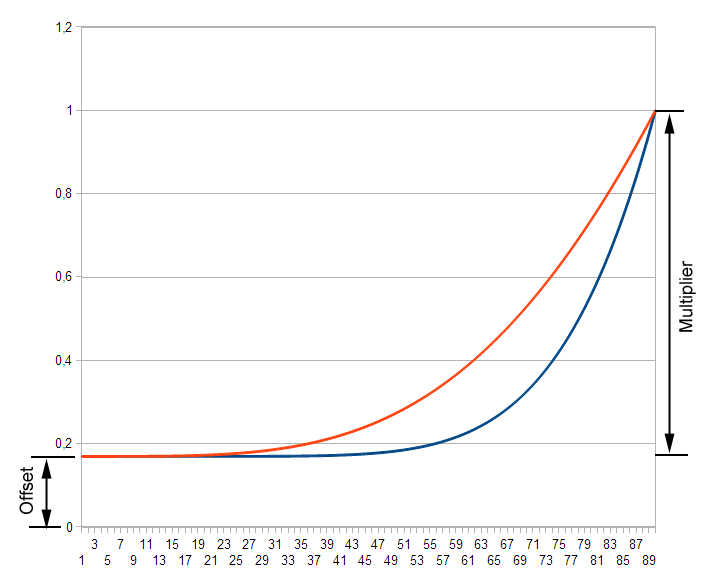
\includegraphics[width=0.6\textwidth]{curves.png}
	\caption{Plot}
\end{figure}

\newpage

\section*{Reflection Model}

Here is an image about the reflection model used in D3D9Client

\begin{figure}[h]
	\centering
	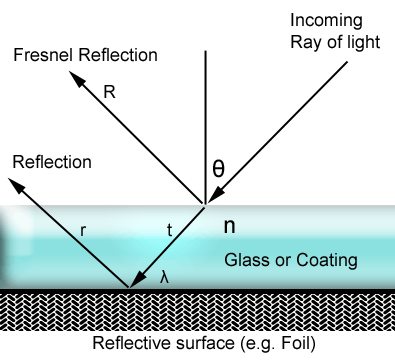
\includegraphics[width=0.35\textwidth]{Fresnel.png}
	\caption{Model}
\end{figure}

The model consists from a fresnel reflection $R$ and a metallic reflection $r$. The lambda $\vec{\lambda}$ is a reflectivity color of the material. $t$ is a fraction of the incoming ray that is not reflected away from the interface. Value of $t$ is simply $t=1-R$.

The intensity of "metallic" reflection alone is independent from a viewing angle. However, when combined with a fresnel reflection it is given by

\begin{equation}
 \vec{r} = \vec{\lambda}(1-R)
\end{equation}

The total reflected light is of course $r+R$. I suppose the fresnel reflection could take a specular color $\vec{s}$ but currently it is considered to be white $\vec{s}=[1,1,1]$

\begin{equation}
\vec{R_{tot}} = \vec{\lambda}(1-R)+\vec{s}R
\end{equation}

The color intensity of the diffuse surface is attennuated by the reflection intensity factor $1-|\vec{\lambda}|$. Resulting pixel color $\vec{c}$ is given by following equation where $\vec{d}$ it the color of the diffuse surface or a texture. 

\begin{equation}
\vec{c} = \vec{d}(1-|\vec{\lambda}|) + \vec{\lambda}(1-R) + \vec{s}R
\end{equation}

In the D3D9Client we simplify the computations and we do not apply fresnel equations to incoming sunlight. A diffuse surface under a reflective coating is considered to be fully lit by the sunlight and other light sources. 

If we would take it in to account then the equation would become

\begin{equation}
\vec{c} = \vec{d}(1-|\vec{\lambda}|)[1-R_0-m(1-\cos\sigma)^p] + \vec{\lambda}(1-R) + \vec{s}R
\end{equation}

Where $\sigma$ is the normal/sun angle.

\end{twocol}
\end{document}
